\chapter{Background}
\label{chapBackground}
M-dwarfs are the most common type of star in our galaxy (excluding brown dwarfs, around 75\% of stars; \citealt{2007Tarter}). Compared to our G-class sun, M-dwarfs are smaller (R $<$\,0.6\,$R_{\odot}$; \citealt{2009Kaltenegger}), cooler (T\,$<$\,4000 K; \citealt{2009Kaltenegger}) and less massive (M\,$<$\,0.6 $M_{\odot}$; \citealt{2009Kaltenegger}). This places them near then red end of the main sequence on a Hertzsprung-Russell diagram (Figure \ref{HRFig}).\\

Due to their low mass, low temperature, and high opacity, convection is the dominant method for transferring energy out from their core. This means that helium will be transported, via convection, further into the envelope than in hotter stars. This convective mixing and the stars low luminosity means the hydrogen burning phase is much longer than in most stars, which leads to an overall greater lifetime. Stars with masses $<$\,0.8\,$M_{\odot}$ will continue to burn hydrogen for longer than the current age of the universe and therefore most will have not currently evolved past the main sequence \citep{1997Adams}. Additionally, the gain in mean molecular weight is very slow \citep{2007Tarter} and this means the luminosity of the star will remain relatively constant for much of its main sequence lifetime. They also undergo a significant period of stellar activity (including flares and sunspots) while they are young.\\

\begin{figure}[!ht]
\centering
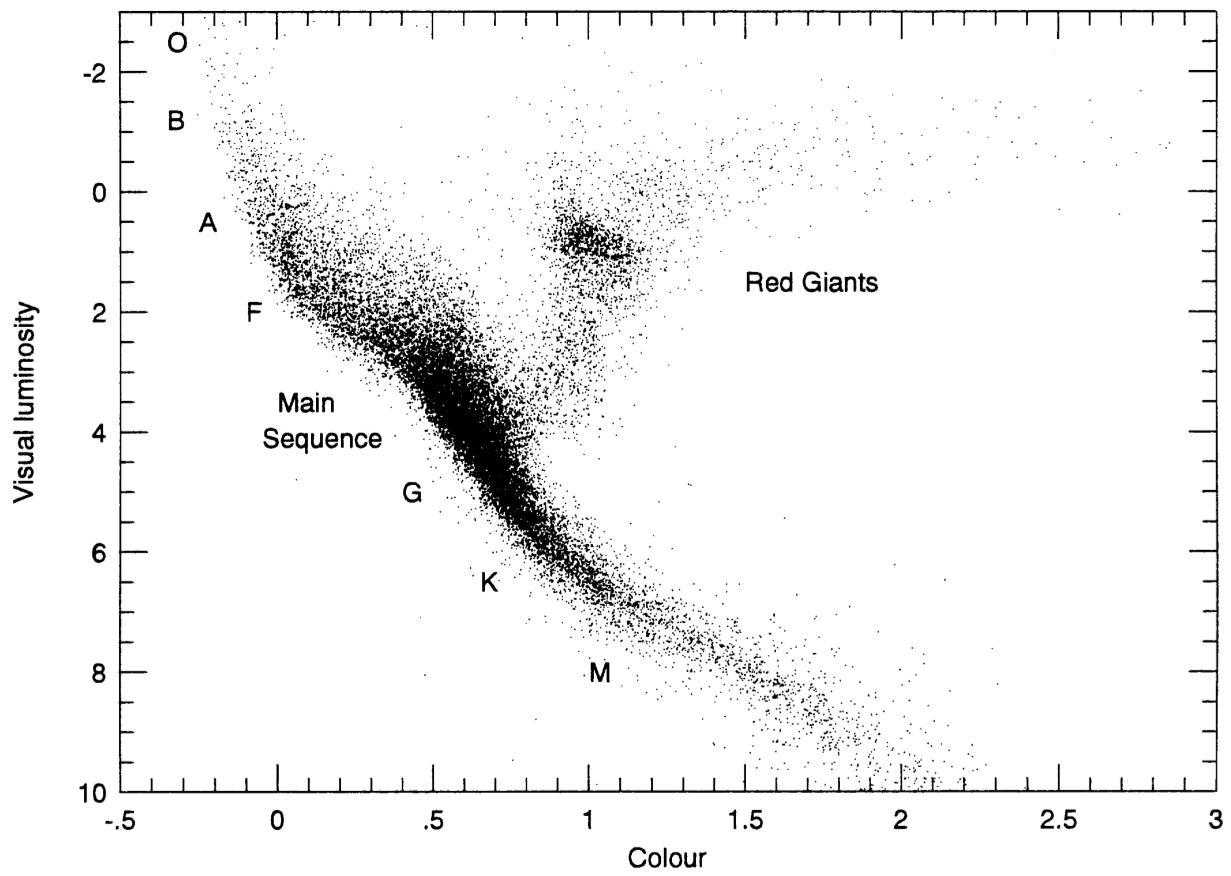
\includegraphics[width=\textwidth]{HRDiagram.png}
\caption{A Hertzsprung Russell diagram, taken from \citet{2005Reid}.}
\label{HRFig}
\end{figure}


Early M-dwarfs are some of the slowest rotating stars. \citet{2009Jenkins} studied the rotational velocities of M-dwarfs and found that from M0 to M3, the median rotational velocity (3.7 kms$^{-1}$ with a variance of 0.9 kms$^{-1}$) did not increase by a significant amount. From M4 to M9.5 the median rotational velocity decreases with temperature, peaking at 9.0 kms$^{-1}$ with a variance of 8.3 kms$^{-1}$.\\

\begin{figure}
\centering
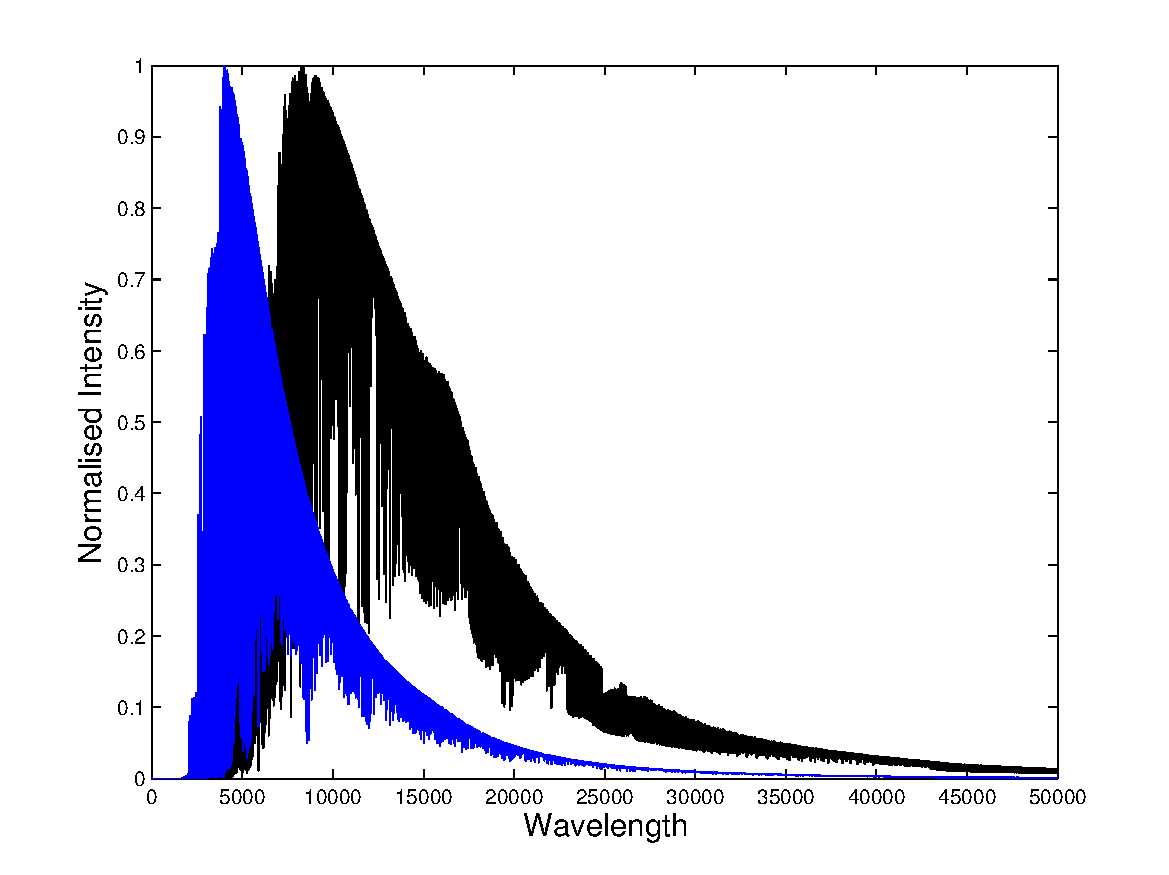
\includegraphics[width=\textwidth]{synth.pdf}
\caption{Normalised synthetic black body spectra of an M-dwarf at 3400K (black) and a G-dwarf at 5800K (blue). Produced using PHOENIX code. The peak energy distribution is located at longer wavelengths than in hotter stars, resulting in a cooler surface temperature.}
\label{FigSynth}
\end{figure}
When the Morgan-Keenan-Kellman (MKK) system of stellar classification was being developed \citep{1943Morgan} in the 1940's, the power and precision of the instruments used limited the study of M-dwarfs to bright candidates. Due to this, only M0-M2 stars were part of that classification scheme. Two additional M-dwarf specific systems developed during this time were the Yerkes system \citep{1938Morgan,1942Kuiper} and the Mt Joy system \citep{1947Joy}. As these systems were widely used, often a star would have multiple classifications. Attempts at a full classification for M-dwarfs were based around red wavelengths due to the majority of the energy distribution coming from those wavelengths (see Figure \ref{FigSynth}). Molecular lines were also used as identifiers of M-dwarf characteristics. These classification systems fell short due to limited capabilities of the equipment at the time. During the early 1990's, detectors that were more red sensitive (for example CCD's) were developed and eventually a unified classification system was established by Kirkpatrick, Henry \& McCarthy \citep{1991Kirkpatrick}. They used a spectrophotometric least-squares comparison of low resolution spectra of 77 stars from 6300-9000 \AA, which covers a number of TiO and VO bands, against standard spectra. Table \ref{TabMsub} gives some of the expected physical physical parameters for M-dwarf subtypes.
\begin{table}[!h]
\centering
\begin{threeparttable}
\caption{M-dwarf physical characteristics for each subclass. Taken from \citet{2009Kaltenegger}.}
\begin{tabular}{| c | c | c | c | c | c | c | c | c | c |}
\hline
SpTy & T & R & Mass & L/100 & M$_{V}$ \\
Dwarf & (K) & (R$_{sun}$) & (M$_{sun}$) & (L$_{sun}$) & (mag) \\
\hline
M0 & 3800	& 0.62 & 0.60 & 7.2 & 9.34 \\
M1 & 3600	& 0.49 & 0.49 & 3.5 & 9.65 \\
M2 & 3400	& 0.44 & 0.44 & 2.3 & 10.12 \\	
M3 & 3250	& 0.39 & 0.36 & 1.5 & 11.15 \\
M4 & 3100 & 0.26$^a$ & 0.20 & 0.55 & 12.13 \\	
M5 & 2800	& 0.20 & 0.14 & 0.22 & 16.0 \\
M6 & 2600 & 0.15 & 0.10 & 0.09 & 16.6 \\
M7 & 2500	& 0.12 & ~0.09 & 0.05 & 18.8 \\	
M8 & 2400	& 0.11 & ~0.08 & 0.03	& 19.8 \\
M9 & 2300	& 0.08 & ~0.075	& 0.015 & 17.4 \\
\hline
\end{tabular}
\label{TabMsub}	
\begin{tablenotes}
\small
\item \textbf{Note.} $^a$ The original reference, \citet{2005Reid}, states 0.36, but should be 0.26 as shown.
\end{tablenotes}
\end{threeparttable}
\end{table}
\section{Spectra}
\label{secSpectra}
Due to the low temperatures of M-dwarf photospheres, molecules can form that would be destroyed in much hotter stars. Strong bands of the diatomic molecule titanium oxide, TiO and vanadium oxide, VO, are quite abundant in the optical regions while carbon monoxide and H$_{2}$O spectral features are dominant in the infrared \citep{2007Tarter,1943Morgan}. Metal hydrides, such as MgH, FeH and CaH appear weakly in early M-dwarfs and gain strength in later subtypes \citep{2005Reid}. Titanium oxide follows a similar pattern, increasing in strength with later spectral types, up to M6 \citep{2005Reid}. Vanadium oxide lines occur predominantly from M7 onwards and blanket the Fe \,\textsc{i} and Ca \,\textsc{ii} lines seen in K and early M dwarfs.\\

\begin{figure}
\centering
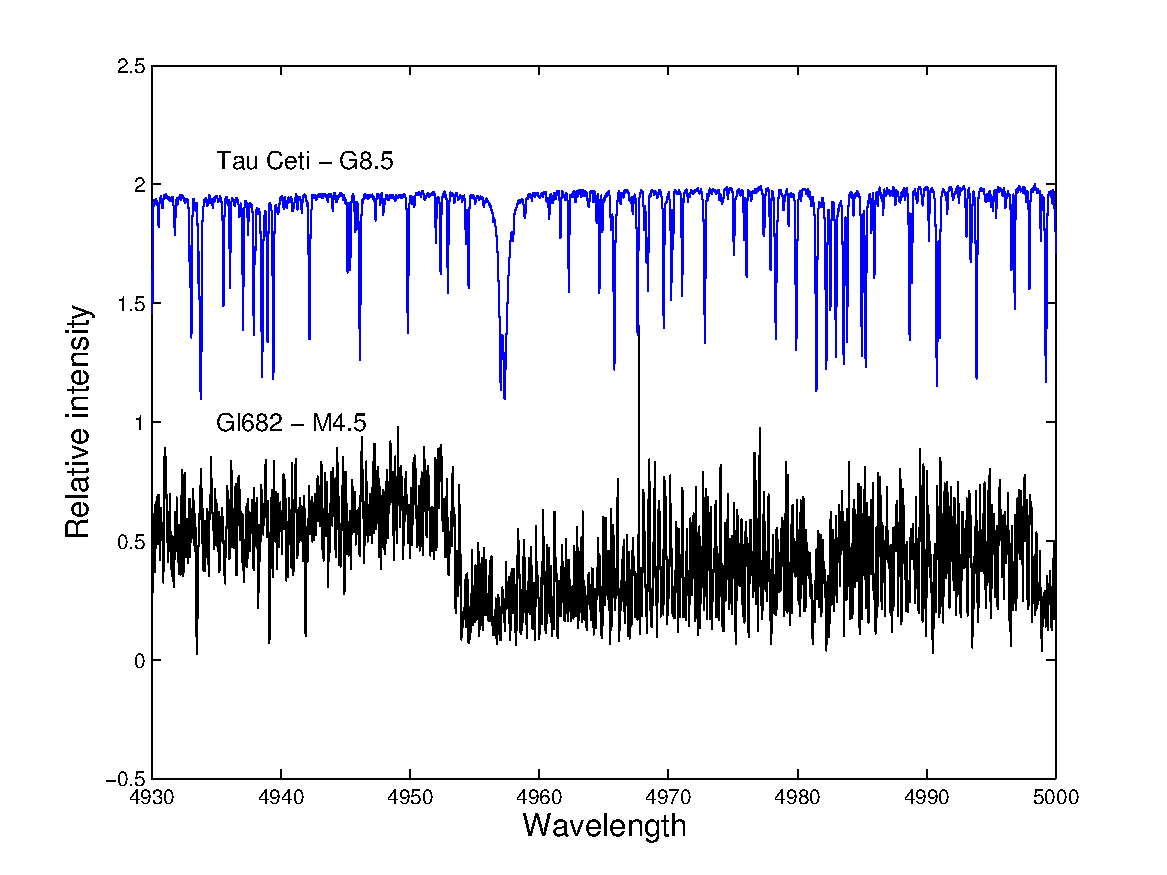
\includegraphics[width=\textwidth]{TauCetiGl682_comparison.pdf}
\caption{Spectra of a G4.5 star, Tau Ceti, and a M8.5 star, Gl682.}
\label{FigSpec}
\end{figure}
These lines appear as molecular bands which require extremely high-resolution spectra to resolve. An example of a bandhead can be seen in Figure \ref{FigSpec}, where a TiO bandhead starts $\sim$4955\,\AA, decreasing in intensity towards redder wavelengths. These absorption bands are stronger in intensity for later subtypes than earlier ones. Additionally, these tightly packed ``forests'' of absorption lines make it difficult to reliably locate the continuum.\\
\subsection{Line Broadening}
\label{SecBroad}
The profile of the absorption lines in a stars spectra can tell us much about the star. In particular, the excitation lifetime of an atom is affected by several natural phenomena that, due to Heisenberg's uncertainty principle, will increase the uncertainty of the energy emission. This will result in a broad distribution of energy absorbed from an atom, which presents as a broad line profile. The stronger these phenomena, the wider and shallower the lines.\\

These phenomena produce several broadening profiles that combine to form the shape of the absorption line seen in the spectra. These include:
\begin{itemize}
\item{Pressure/collisional broadening - produced from the collision of atoms. Atoms that were absorbing a photon at the time of the collision would experience an interruption in the excitation process. This interruption, across all the atoms of a particular species, result in a Lorentzian energy distribution.}
\item{Thermal/Doppler broadening - where the thermal energy of the star will add a random motion to the velocity of the atom. The radial component of this motion will be different for each atom and the combination of all atoms radial motion will produce a Gaussian profile.}
\item{Rotational broadening - the rotation of the star will cause blueshift and redshift from the atoms moving radially towards and away from us. The higher the rate of rotation, the greater the shift, and the broader the resulting energy distribution.}
\item{Microturbulence - a non-thermal, Gaussian broadening that operates on small scales and is affected by effective temperature and surface gravity \citep{2007Montalban}.}
\item{Macroturbulence - the convective zone of a star is granularised, with a range of  radial velocities for each granule. Unlike the previous broadening effects, this broadens the ``wings'' of the line, rather than the ``body''.}
\end{itemize}

Due to the low temperatures of M-dwarfs, absorption lines are minimally effected by temperature broadening, however some M-dwarfs can have significant rotational velocity, which can strongly influence the width of the lines present.\\

\begin{figure}
\includegraphics[width=\textwidth]{RotBroad.jpg}
\caption{Comparison image of two M-dwarfs, one a fast rotator (blue) and one a slower rotator (green), highlighting the effect of rotational velocity. The absorption lines comprising the CO bandhead from $\lambda > 2.3226\,\mu$m can be seen to be strongly blended due to rotational broadening in the blue spectra (vsin(i)\,=\,29.8\,kms$^{-1}$), while the green spectra's lines are much more resolvable. Figure taken from \cite{2018Kesseli}}
\label{FigRotation}
\end{figure}
Comparison of spectra from two different stars (Figure\,\ref{FigRotation}), one with high rotational velocity (blue) and another with a slower velocity (green), highlight the influence of rotational broadening. The lines comprising the CO bandhead in the faster rotator have been broadened to the extent that it is impossible to resolve any individual line as they have blended into one feature. The slower rotator, however, has lines that are less broadened and thus can be resolved.\\

\begin{figure}[!ht]
\includegraphics[scale=0.8]{LimbDarkening.eps}
\caption{Diagram highlighting the limb darkening effect. Due to the opacity of a star, photons emitted from the centre of the stellar disk will come from a hotter, deeper layer of the photosphere than photons from the edge. For a specific optical depth (black arrows) photons will be emitted from a warmer depth (the red dotted line) in the centre, than from the edges (the blue line).}
\label{FigLimb}
\end{figure}

One additional effect on the shape of an absorption line comes from limb darkening. The opacity of a star means that only light down to a certain depth will escape the star. The flux collected by a telescope will be the radial component of all the light emitted by the star that is parallel to line of sight. Of this light, the photons coming from the centre of the disk will come from a deeper, and therefore hotter region of the star than from the edges.\\

\section{Photometry and colour}
\label{SecPhotCol}
Photometry can provide complimentary information to spectroscopy. A star's flux in two different passbands will vary and the difference between the corresponding magnitudes from those passbands is known as a colour, e.g. J-H, W1-W2 etc. Previous work have identified relationships between classes of stars and photometric colours. These relationships link colours to physical characteristics of stars, such as temperature and gravity which can be used to highlight the colour ranges that a particular type of star will inhabit. These relationships are seen in plots of two different colours, in which the x-axis colour is sensitive to temperature, while the y-axis colour is a measure of surface gravity. As different classes of stars will have different temperatures and surface gravities, their location in a colour-colour plot is expected, in a perfect world, to be unique. As stars evolve, the changes they undergo are seen in their movement across a colour-colour diagram (just like a Hertzsprung-Russell diagram). Figure \ref{FigCol} is an example of a colour-colour plot. The branch between 0 $<$ H-K $<$ 0.2 are predominantly main sequence A, F, G \& K stars, which then separate into two branches at higher H-K values. The upper branch, represented by the dashed line, are populated by stars that have evolved into giants. The lower branch represented by the solid line are M-dwarfs that are still in the main sequence. Knowledge of how a particular colour corresponds to temperature or gravity can provide us with information about a particular star or the make-up of a group of stars.\\

\begin{figure}[!t]
	\centering
	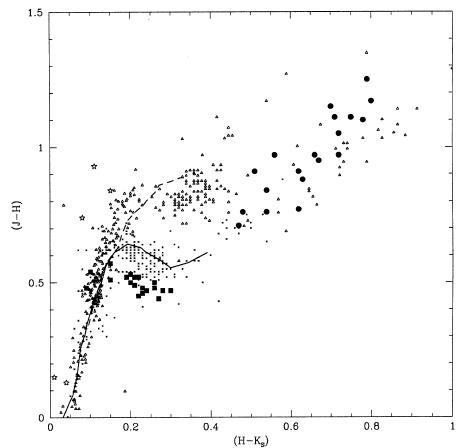
\includegraphics[width=\textwidth]{FigCol.jpg}
	\caption{A colour-colour diagram highlighting the different evolutionary paths dwarfs and giant stars will take. Taken from \citet{2005Reid}.} 
	\label{FigCol}
\end{figure}
The challenge in finding relationships that define M-dwarfs is that due to photometric confusion, a stars photometry can be `scattered', expanding the boundary of the colour region a class inhabits, which can overlap with a neighbouring class. For example, it is important to define strong boundaries between M-dwarfs, and K and M giants (red, cyan, and green respectively). Also late K stars (dark blue) and early L stars (not shown), which occur at colour values just before and just after the M-dwarf branch, can have similar colour characteristics to M-dwarfs and therefore need to be excluded from any selection criteria produced. Selecting a colour region where the M-dwarfs are expected to inhabit will also include these non-M-dwarfs, which are termed contaminates. Certain colour planes can have advantages over others. One colour plane might position a specific class of contaminates further away (in colour-colour space) from the M-dwarfs than other colours which will reduce their contribution to the levels of contamination. For example, Figure \ref{FigHK} has significant overlap of K-stars and the M-dwarfs span a small colour range ($\sim$0.15). The M-dwarf/K-star overlap is reduced in the J-K, W1-W2 colour plane of Figure \ref{FigW1W2} and spans a much larger colour range ($\sim$0.25).\\
\begin{figure}
	\centering
	\subfloat[]{\label{FigHK}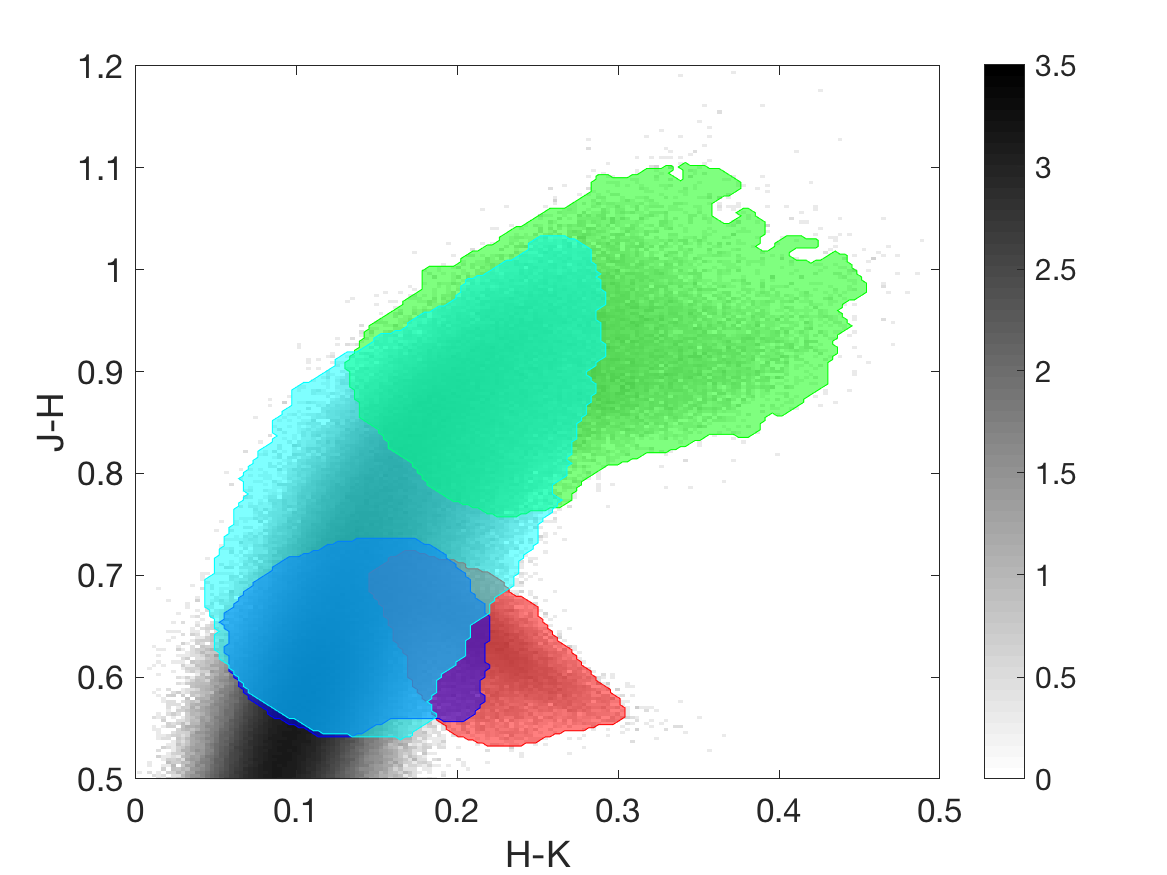
\includegraphics[width=0.6\textwidth]{JH-HK.png}}
	\subfloat[]{\label{FigW1W2}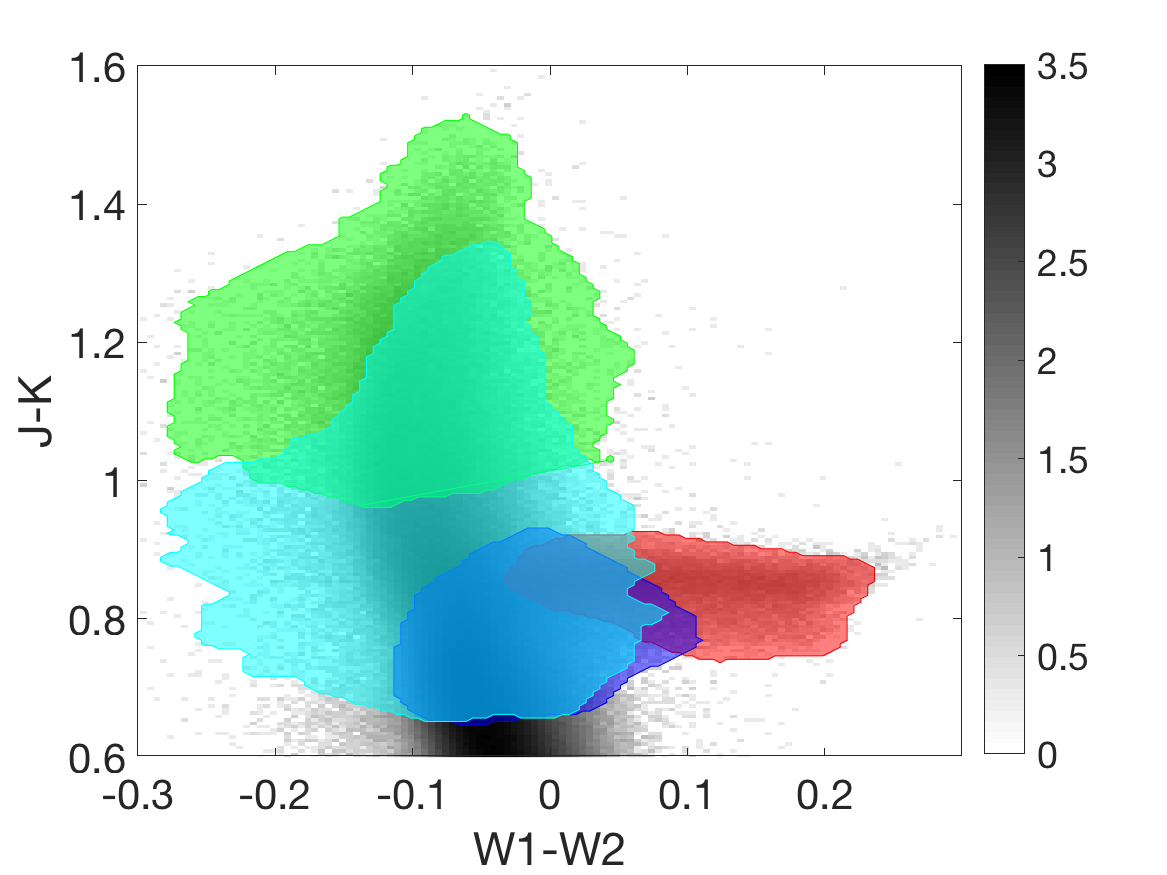
\includegraphics[width=0.6\textwidth]{JK-W1W2.png}}
	\caption{Colour-colour diagrams comparing the distributions of: Red - M-dwarfs; Blue - K-dwarfs; Cyan - K-giants; Green - M-giants.}
	\label{FigColComp}
\end{figure}
\section{Exoplanet Detection}
Improvements in technology have allowed us to detect fainter objects than we could previously. However, we are unable to observe most exoplanets in the same way we observe stars. The majority of light coming from an exoplanet is reflected light from its host star. In most cases this is not sufficient to distinguish the exoplanet from the star. Indirect methods of gaining information, through observing the influence of the exoplanet on the host star, are much more successful. The two most common methods are Doppler spectroscopy and planetary transits.
\subsection{Doppler spectroscopy}
\label{SecRV}
A star system with orbiting exoplanets has its barycentre offset from the rotational axis of the star. The effect of this is that the star moves in a very small orbit, which is detectable via periodic changes in the Doppler velocity of the star. High-resolution spectra of the star will show a shift in the wavelength of spectral lines, proportional to the amount the star is moving radially towards or away from the Earth. As the star goes through its orbit, this Doppler velocity will vary periodically. By measuring this change in the Doppler velocity, the minimum mass of an exoplanet can be calculated.\\
\begin{equation}
K = \sqrt{\frac{G}{1-e^2}} m_p sin(i) (m_\ast + m_p)^{-1/2} a^{-1/2}
\label{EqRV}
\end{equation}
The exoplanet's mass, $m_p$, is derived from the Doppler velocity variation amplitude, $K$, through Equation \ref{EqRV}. $G$ is the gravitational constant, $e$ is the orbital eccentricity, $i$ is the angle between the orbital plane and a reference plane perpendicular to the line of sight (see Figure \ref{FigOrbit}), $m_\ast$ is the mass of the star and $a$ is the semi-major axis. As an example, the Earth effects a Doppler velocity of 0.09 m s$^{-1}$ and Jupiter contributes a value of 12.7 m s$^{-1}$ to the Sun.\\
\begin{figure}
\centering
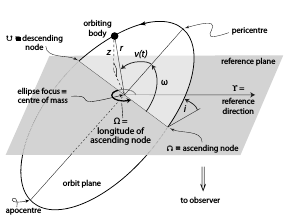
\includegraphics[width=\textwidth]{ExoOrbit.png}
\caption{Diagram showing the orbital elements of an exoplanet orbiting a star. Taken from \citet{2011Perryman}.}
\label{FigOrbit}
\end{figure}
This method has some limitations. Firstly, we see a fraction of the total Doppler velocity as our measurements are dependent on the orbital inclination of the system. Due to this, when we measure the mass of the exoplanet, we obtain an estimate of the minimum mass, m$_p$ sin(i), not the total mass. We would be unable to detect the movement of stars whose orbital inclination is at $0^{\circ}$ and therefore unable to detect the presence of exoplanets by this method.\\

Doppler spectroscopy benefits from systems where the orbital radius of the exoplanet is close to the star. The Doppler velocity variation amplitude is dependent on the orbital radius so a close-in exoplanet would produce a larger amplitude in Equation \ref{EqRV} than if it were further out. Spectra that have a large number of deep and very narrow absorption lines give highly accurate radial velocity results. As such, cooler stars (such as M-dwarfs) are very suitable due to the large number of molecular lines and low amount of line broadening due to their typically slow rotation speed \citep{2005Reid}. The first exoplanet to be detected orbiting a main sequence star, 51 Pegasi, was detected using this method \citep{1995Mayor}. Since that time hundreds of exoplanets have been detected using Doppler spectroscopy.
\subsection{Transits}
\label{SecTrans}
Another way to detect exoplanets is to observe a periodic drop in light coming from the star when the exoplanet passes in front of the star from our perspective. A photometric series is obtained over a period of time large enough to assure several orbits of the planet. Looking at Figure \ref{FigTransit}, you can see that the flux from the system is a combination of the luminosity of the star and light reflected from the exoplanet. As the exoplanet moves in front of the star, it obscures an area of the visible face of the star, blocking the contribution to the received flux from that area. This causes a drop in the flux that will increase to its original level once the exoplanet is no longer obscuring part of the star. A smaller secondary dip can be seen when the exoplanet is behind the star and its reflected light is obscured by the star.\\
\begin{figure}[hbt]
\centering
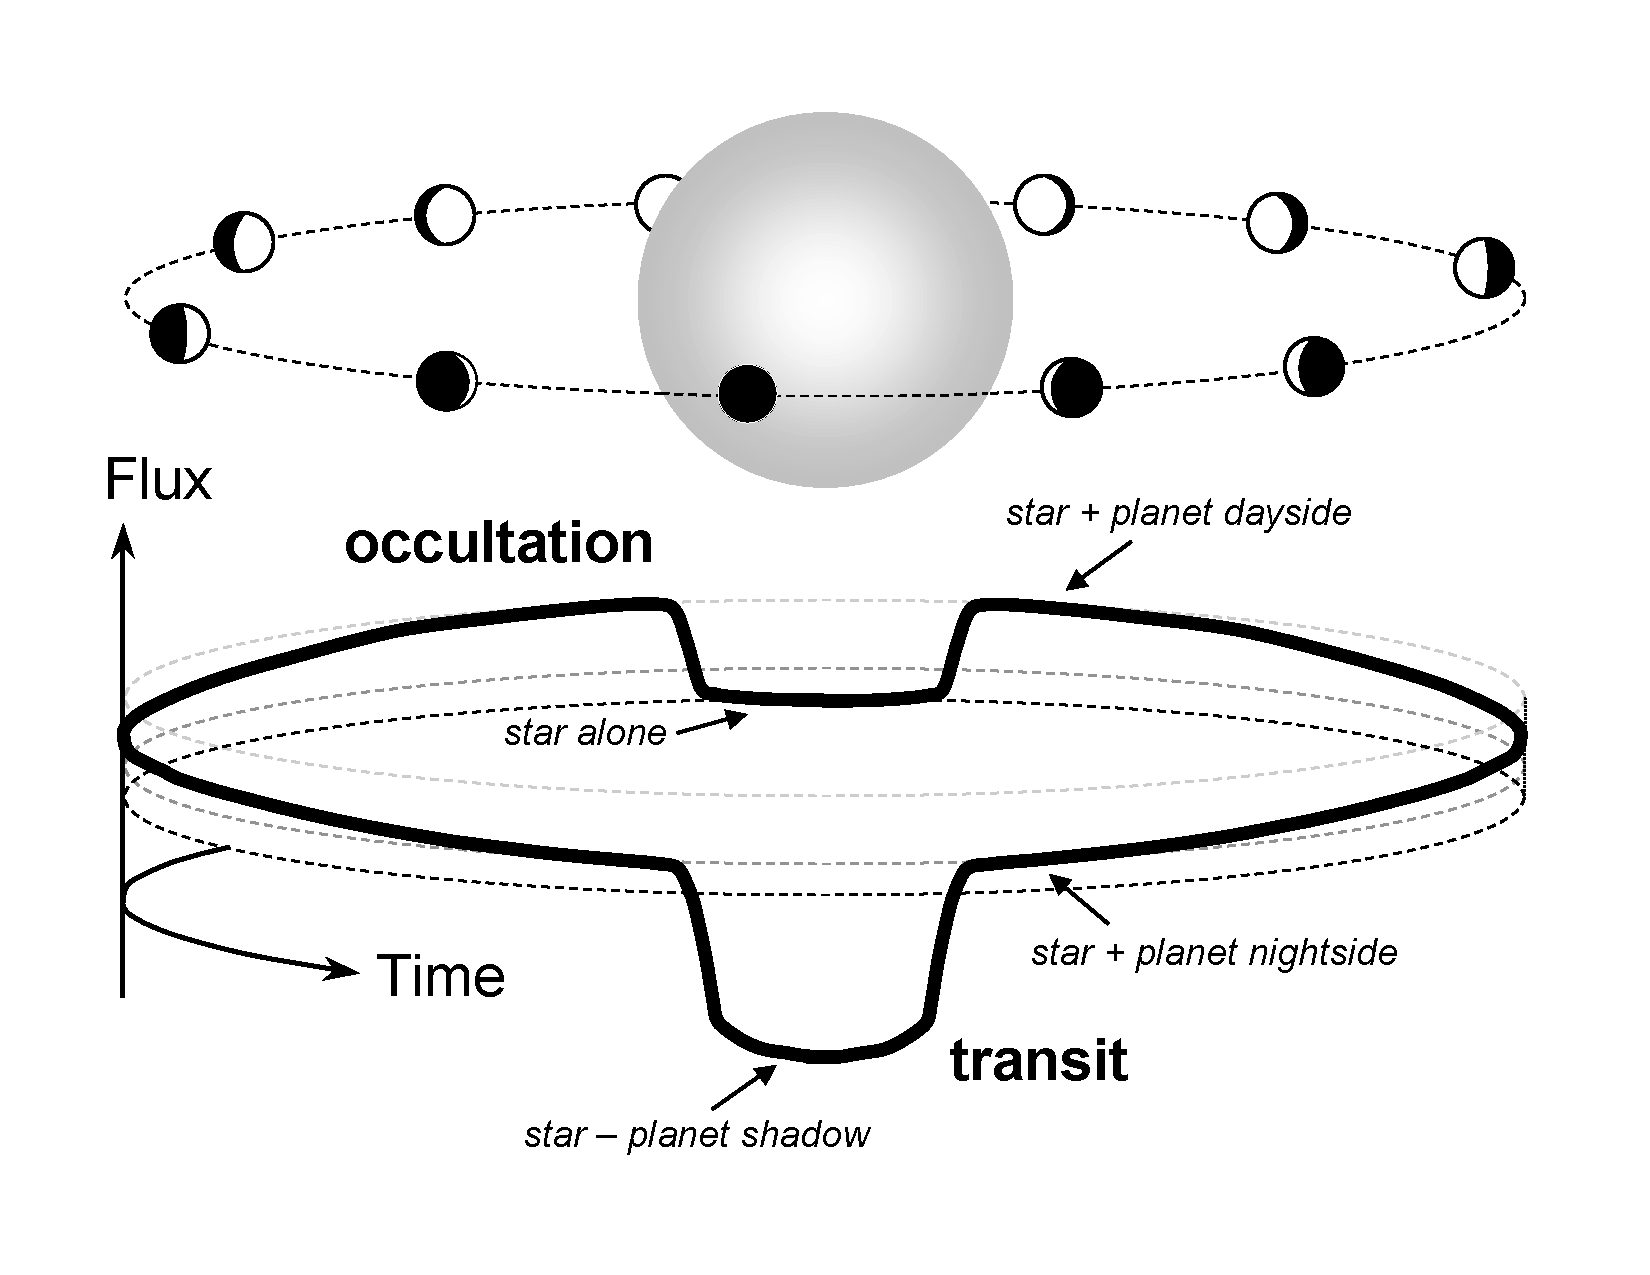
\includegraphics[scale=0.4]{circular_diagram.pdf}
\caption{Diagram showing the effect on the luminosity of a star when an exoplanet passes across the visible face of the star. Taken from \citet{2010Winn}.}
\label{FigTransit}
\end{figure}
The drop in flux is directly proportional to the ratio of the exoplanetary and stellar radii, as can be seen by Equation \ref{EqFluxDrop}, where $R_p$ and $R_\ast$ are the radii of the exoplanet and the star, respectively. By obtaining spectra of the star, an estimate of the radius of the star can be obtained and therefore, an estimate of the planetary radius.\\
\begin{equation}
\Delta F = \left(\frac{R_p}{R_\ast}\right)^2
\label{EqFluxDrop}
\end{equation}
While Doppler spectroscopy can be performed on systems with a range of orbital orientations, an observable transit requires an orbital orientation close to edge-on ($i \approx 90^\circ$). The actual distribution of orbital inclinations will range from $0^\circ$ to $90^\circ$. Assuming randomly distributed orbital orientations and circular orbits, the probability that a given system will have an exoplanet transit will be observable can be calculated from Equation \ref{EqTrans}.
\begin{equation}
P_{transit} = \frac{R_\ast + R_p}{a}
\label{EqTrans}
\end{equation}
The probability of detecting the transit of a Sun-Earth system is 0.47\%, meaning we would need to observe, on average, 200 similar systems to find one that is transiting. Exoplanets orbiting close to their host star, such as habitable zone exoplanets around M-dwarfs, are more likely to transit than those further out (see Section \ref{SecHab}). An Earth size exoplanet orbiting within the habitable zone of an M7 star (a = 0.35 au) gives a probability of $\sim$2.0\%.\\

As well as having a higher probability of transiting, the closeness of the habitable zone in M-dwarfs is an advantage to transit detection as any suitable exoplanets will have short orbital periods and so photometry of multiple orbits can be obtained over a shorter period of time than exoplanets further out. Additionally, due to their low-mass and correspondingly smaller radii, M-dwarfs do not need as high precision photometry for a detection since the exoplanet-to-star radius ratio is larger and therefore the transit depth is deeper \citep{2011Lepine}.
\section{Observational surveys}
There has been (and will continue to be) many observational surveys that have detected the presence of exoplanets and obtained their characteristics. The majority of these use spectra to obtain Dopler velocities (\ref{SecRV}) and photometry to obtain transit information (\ref{SecTrans}).
\subsection{Spectroscopic surveys}
\label{SecSpecSurveys}
Exoplanet focused spectroscopic surveys obtain radial velocities to detect the presence of exoplanets around a host star. Spectroscopes with high resolution and stability provide more accurate measurements of radial velocity, allowing for the detection of lower mass exoplanets. There are many surveys that build their spectroscopes with a focus on resolution and stability to obtain the accuracy desired. The most important current and upcoming exoplanet surveys are HARPS, LAMOST and FunnelWeb.\\

Some of the most accurate Doppler velocities in recent time have come from the European Southern Observatories (ESO) High Accuracy Radial velocity Planet Searcher (HARPS; \citealt{2003Mayor}) spectrograph using the 3.6m telescope at La Silla, Chile. HARPS is a fibre-fed, cross-dispersed echelle spectrograph that was designed to be highly stable, allowing for Doppler velocities with precision of down to 1ms$^{-1}$. The spectroscope is placed inside a vacuum chamber which reduces the amount of spectroscopic line drift from atmospheric pressure changes to less than 0.1 ms$^{-1}$ \citep{2004Rupprecht}. Additionally the temperature of the chamber is kept stable to 0.01 K over a year, and simultaneous Thorium-Argon calibration is used.\\

The Large Sky Area Multi-Object Fiber Spectroscopic Telescope (LAMOST; \citealt{2012Cui}) survey uses the Guo Shou Jing telescope to obtain medium resolution (R = 1000-1500) spectra of up to 10 million northern hemisphere ($\delta \geq 10\degree$) objects in the Milky Way. With a field of view of 5$\degree$ and 4000 optical fibres, the scientific goal was to obtain large numbers of spectra over a short timescale.\\

FunnelWeb (Raines et al, in prep) is an upcoming spectroscopic survey that, unlike most surveys that focus on one star at a time, will observe up to 300 stars simultaneously. It will use the TAIPAN spectrograph \citep{2014Kuehn} on the Australian Astronomical Observatory's (AAO) UK Schmidt Telescope to obtain high quality (S/N $\sim$ 100) spectra, at a wavelength range 3700\,-\,8700$\hbox{\AA}$ and a resolution of R $\geq$ 2000, of around 2 million southern hemisphere ($\delta \leq 0\degree$) stars down to {\em Gaia} G = 14.5. TAIPAN uses 150 robotically controlled optical fibres, called ``Starbugs'', to observe selected stars within a 6\degree region of the sky. A typical observing night will consist of several ``tiles'' -- sections of sky in which the objects of interest have been identified and an automated system will determine the positioning of each starbug and the path a starbug will have to move to get to its new position when transitioning from one tile to the next. The main goals of the survey include a spectral library with detailed stellar parameters (including T$_{\rm eff}$, log(g), [Fe/H] and [$\alpha$/Fe]), including stellar spectra for targets being observed by TESS (see Section\,\ref{SecPhotSurveys}), with M-dwarfs a particular focus. 
\subsection{Photometric surveys}
\label{SecPhotSurveys}
Photometric surveys measure the intensity of light across particular wavelength regions (passbands). The total flux across each passband, $f$, is converted into an apparent magnitude, $m$, using Equation \ref{EqFlux}, where C is a zero-point constant which is specific to each passband.\\
\begin{equation}
m = -2.5\,log_{10}(f)\,+\,C
\label{EqFlux}
\end{equation}

Comparison of two stars apparent magnitudes is problematic as a bright star, far away, can appear similar to a close, but dim, star. Absolute magnitude, $M$, is the better comparison as it measures the luminosity at a fixed distance -- 10 parsecs. From Equation \ref{EqAbs} it can be seen that both apparent magnitude and distance, $d$, are required. Apparent magnitude requires flux to calculate, which is simple to obtain. However, absolute magnitude requires both apparent magnitude and distance, the latter being something difficult to achieve without a measurement of parallax, which in turn requires multiple, precise measurements of the location of a star on the sky.\\
\begin{equation}
M = -5\,log_{10}(d) + 5 + m
\label{EqAbs}
\end{equation}
Photometric analysis of stars often involves looking at the difference between two photometric magnitudes, known as a colour. For example, the colour B-V is m$_B$\,-\,m$_V$. Colours can be a good proxy for stellar characteristics such as temperature and gravity, especially between stellar subtypes.\\

The photometric surveys that are of particular importance to this thesis are {\em Gaia}, 2MASS, WISE, and TESS. These all-sky surveys provide photometry at a range of optical and near-infrared wavelengths. In particular, as can be seen from Figure \ref{FigPassband}, they probe critical wavelengths for the selection of M-dwarfs, which emit most of their flux between 0.6 nm and 5 $\mu$m).\\

\begin{figure}[!ht]
\hspace{-1cm}
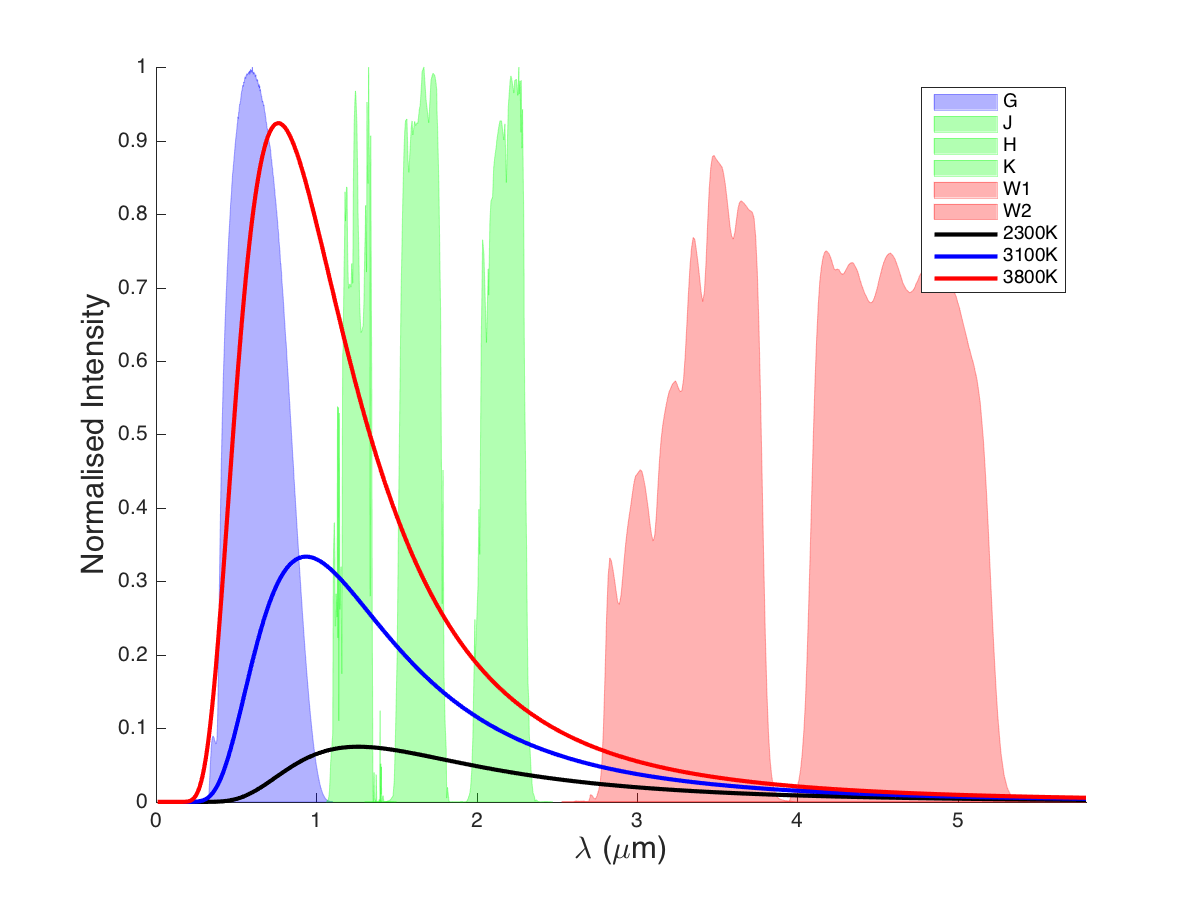
\includegraphics[scale=0.8]{Passbands.png}
\caption{Wavelength coverage of the {\em Gaia} (in blue), 2MASS (in green) and WISE (in red) passbands. Blackbody curves of objects at temperatures corresponding to M0, M4, and M9 are overplotted to highlight the flux coverage across these bands.}
\label{FigPassband}
\end{figure}
The Two Micron All Sky Survey (2MASS; \citealt{2006Skrutskie}) was a ground-based, whole-sky photometric survey that used two 1.3 m telescopes, one in Chile and the other in Arizona, USA to obtain photometry of 470 million objects from 1997 to 2001. Having a telescope in both hemispheres allowed for whole-sky coverage. It obtained photometry in the J, H and K$_s$ passbands (1.2, 1.7 and 2.2\,$\mu$m). The K$_s$ passband stands for ``K-short'' and is a variant on the Johnson K passband that has its upper wavelength limit of 2.4\,$\mu$m reduced to 2.3\,$\mu$m. This limits the contribution of thermal background noise from the Earth in the flux.\\

WISE \citep{2010Wright} is a space satellite that was built by NASA to survey the whole sky at $3.4, 4.6, 12$ and $22 \mu m$ (W1, W2, W3, W4). The four WISE passbands are designed to be sensitive to emissions from different types of objects in the sky. W1 detects flux from stars and galaxies, W2 picks up thermal radiation from internal heat sources. Thermal radiation from asteroids is seen in W3 and W4 is sensitive to dust from star forming regions. As can be seen in Figure \ref{FigPassband}, M-dwarfs radiate sufficient flux in the regions covered by W1 and W2. However, W3 and W4 occur at very red wavelengths, with insufficient flux to provide information about M-dwarf characteristics. Over 7 months in 2010, the WISE satellite obtained photometry of over 563 million objects. The full data set includes basic position information, photometric magnitudes for W1, W2, W3 and W4, and where possible, cross-matched J, H, and K$_s$ magnitudes from 2MASS.\\

{\em Gaia} \citep{2016Gaia} is the successor to Hipparcos and seeks to obtain photometry of approximately 1 billion objects over a 5 year period (2014-2019). It obtains photometry of each object 70 times over this period and from this, highly precise astrometry can be obtained. The light it detects has a coverage of 320-1000\,nm, from which the G passband will be measured. The light is then passed through two fused-silica prisms which separates the light into two other passbands, the Blue Photometer (BP) and Red Photometer (RP) which have 330-680\,nm and 640-1050\,nm wavelength ranges respectively. The precise and frequent measurements mean that highly accurate parallaxes and proper motions can be measured for most, if not all, of the stars it observes. Parallaxes are expected to be obtained with precisions of 9-11\,$\mu$as for stars brighter than V = 10, 10-27\,$\mu$as at V = 15, and 100-350\,$\mu$as at V = 20. Doppler velocities will be obtained for stars brighter than V = 15 with an accuracy of between 1\,-\,15\,kms$^{-1}$.\\

The Transiting Exoplanet Space Satellite (TESS; \citealt{2009Ricker}) was designed as a follow up to the work of the Kepler survey. This will be the leading source of transiting exoplanet detection, especially around M-dwarfs, in the near future. Its focus is high quality, all-sky coverage of around 500,000 stars in the solar neighbourhood, particularly F5-M5 main sequence dwarfs, looking for transiting exoplanets. It will cover a wavelength range of 600-1000\,nm and focus on planetary orbits of around 10 days for most stars, and up to 40 or more days for stars near the ecliptic poles, where longer coverage is possible. Initial predictions expect one super-earth planet (1.25\,-\,2 R$_{\oplus}$) with a planetary orbit of less than 10 days, per 500 stars observed.
\section{Habitability}
\label{SecHab}
The standard measure for finding rocky exoplanets with the potential to support life is known as the ``habitable zone''. The habitable zone of a star is the range of radii that are not so close that a rocky exoplanet would be too hot to support life and not too far that it would be too cold. Specifically it is the range of distances at which a rocky exoplanet can retain liquid water at its surface \citep{1993Kasting}.\\

There are multiple parameters that will determine an exoplanets ability to retain liquid water at its surface, including the exoplanet's orbital radius, environmental characteristics, rotation speed and the mass of the host star. However, the most significant factor is the exoplanet's surface temperature which is primarily dependent on the incident radiation on the exoplanet and therefore, the orbital radius. However, other factors also play a key role in the surface temperature.\\

Stellar radiation incident on a planetary atmosphere will penetrate that atmosphere, be absorbed, and subsequently re-emitted. The re-emitted radiation will have a longer wavelength than the incident stellar radiation. Greenhouse gases such as methane, water, and carbon dioxide, have molecular structures that make them efficient absorbers of near-infrared radiation. Therefore, while an atmosphere may be transparent to incident optical radiation from the star, it could be opaque to re-emitted infrared radiation. The re-emitted radiation cannot therefore escape the atmosphere and the planet is thereby warmed by the presence of these greenhouse gases in the atmosphere. This heating would extend the outer limit of the habitable zone to include exoplanets that would be too cold from stellar radiation alone.\\

Rocky exoplanets orbiting within the habitable zone are not guaranteed to be habitable. Additional factors include the rate of surface impacts, the presence of water, the density of the atmosphere and the presence of greenhouse gases, such as CO$_2$ \citep{2007Selsis}.\\

For a given star system, a range of radii will define the habitable zone and these ranges can vary over time due to the evolution of the star. The habitable zone of the Solar system currently extends from $\sim$ 0.9 to 1.4 AU. Once the Sun ends its hydrogen burning phase, it will evolve into a red giant. During this transition, conditions will extend the inner boundary of the habitable zone past the Earth.\\

Using the habitable zone calculator developed by \citet{2013Kopparapu}, values for the inner and outer edges of the habitable zone for M-dwarfs have been calculated. This model simulates a runaway greenhouse effect - where absorption of reflected infra-red light by greenhouse gases causes a positive feedback loop to occur until the surface temperature has risen sufficiently to evaporate any surface water - on a 1 $M_{\oplus}$ exoplanet. This will have a strong influence on the inner boundary of the habitable zone as distances that would normally be far enough away from the host star to support liquid water, might have that water used in the greenhouse process. As can be seen in Table \ref{TabHZTL}, M-dwarf habitable zones lie close to their host star, which would be expected due to their low luminosity (see Table \ref{TabMsub}). Methods for detecting exoplanets using exoplanetary transits and Doppler velocity variability benefit from a small orbital radius. Conversely, being so close to the star limits habitability due to stellar activity, X-rays and ultraviolet radiation that would require a very strong magnetosphere and ozone layer. As a star ages, its will undergo changes that will alter the flux. This can shift the location of the habitable zone to the point where a exoplanet might lose the conditions necessary to support life. M-dwarfs have a longer main sequence lifetime than hotter stars and their luminosity is relatively constant during this time. Therefore, the habitable zone is more likely to stay at the same location for longer, than in hotter stars.\\
\begin{table}
\centering
\begin{tabular}{|l|l|l|l|l|}
\hline
Spectral& \multicolumn{2}{|c|}{a(HZ)} & \multicolumn{2}{|c|}{t$_{locking}$}\\
Subtype & \multicolumn{2}{|c|}{(AU)} & \multicolumn{2}{|c|}{(M Yr)}\\
\cline{2-5}
 & Inner & Outer & Inner & Outer\\
\hline
M0 & 0.277 & 0.529 & 455.3 & 22090\\
M1 & 0.194 & 0.374 & 80.56 & 4135\\
M2 & 0.157 & 0.307 & 28.07 & 1569\\
M3 & 0.127 & 0.250 & 11.75 & 683.5\\
M4 & 0.077 & 0.153 & 1.891 & 116.4\\
M5 & 0.049 & 0.098 & $<$ 1 & 16.40\\
M6 & 0.031 & 0.064 & $<$ 1 & 2.493\\
M7 & 0.023 & 0.048 & $<$ 1 & $<$ 1\\
M8 & 0.018 & 0.037 & $<$ 1 & $<$ 1\\
M9 & 0.013 & 0.026 & $<$ 1 & $<$ 1\\
\hline
\end{tabular}
\caption{Estimated habitable zone radii and tidal locking timescales for a 1 Earth mass exoplanet around an M-dwarf.}
\label{TabHZTL}
\end{table}
\begin{figure*}[t!]
\centering
\includegraphics[width=\textwidth]{TidalBulge.jpg}
\caption{Diagram of the effect of tidal forces on an star from an exoplanet. The dotted line is the spherical shape the star would have if not for tidal forces. The shaded region are the bulges caused due to the gravitational influence of the exoplanet on the star. The attraction between the exoplanet and near bulge (A) is stronger than with the far bulge (B). This induces a torque which will slow the stars rotation and transfer angular momentum to the exoplanet. A similar process will occur on the exoplanet from the stars gravitational influence. Taken from \citet{2011Perryman}}
\label{FigTidal}
\end{figure*}
The gravitational influence of a star on an exoplanet will not only constrain the motion of the exoplanet to an orbit around the star but also affect its shape and rotation, due to tidal effects, resulting in a localised distortion of the surface of the exoplanet that moves along the orbital plane as the exoplanet rotates. A torque is generated via the distorted shape which will reduce the rotational angular momentum of the exoplanet and increase the orbital angular momentum. If the rotation period reduces sufficiently to synchronise with the orbital period, the exoplanet will experience tidal locking - where one side of the exoplanet is constantly facing the star and the other side will be permanently dark. Instances of tidal locking exist in our solar system e.g. between the Earth and the Moon and Pluto and Charon.\\
\begin{equation}
t_{lock} \approx \frac{wa^6IQ}{3Gm_p^2kR_p^5}
\label{EqTidal}
\end{equation}
The time an exoplanet would take to tidally lock with its host star can be estimated using Equation \ref{EqTidal}, taken from \citet{1977Peale}, where $w$ is the spin rate of the exoplanet, $a$ is the semi-major axis of the orbit, $I$ is the moment of inertia, $Q$ is the rate at which the orbiting satellite can dissipate the tidal energy, $G$ is the gravitational constant, $m_p$ is the mass of the exoplanet, $k$ is the love number and $R_p$ is the radius of the exoplanet. Values for $Q$ and $k$ are obtained as a ratio. Accurate values are difficult to obtain, even for nearby planets. For example, Earth values of $Q$, which are easier for us to obtain than any other planet, range from 90 to 500 \citep{1996Ray}. Using the habitable zone radii taken from Table \ref{TabHZTL} and assuming Earth values for the exoplanet, estimated M-dwarf tidal locking times for habitable exoplanets are presented in Table \ref{TabHZTL}. Tidal locking is generally considered bad for habitability as one half of the exoplanet will be irradiated constantly while the dark side would receive no direct starlight and thus be too cold to support life. Recent models have shown, however, that while tidal locking makes habitability more complicated, it is not as restrictive as initially thought \citep{2013Yang}. Tidal forces increase cubically with decreasing distance so the closer the exoplanet is to the star, the higher the tidal force. Since the habitable zone of M-dwarfs are generally close to the host star, the chances of tidal locking are greater than for habitable planets orbiting hotter stars.\\
\begin{figure}
\centering
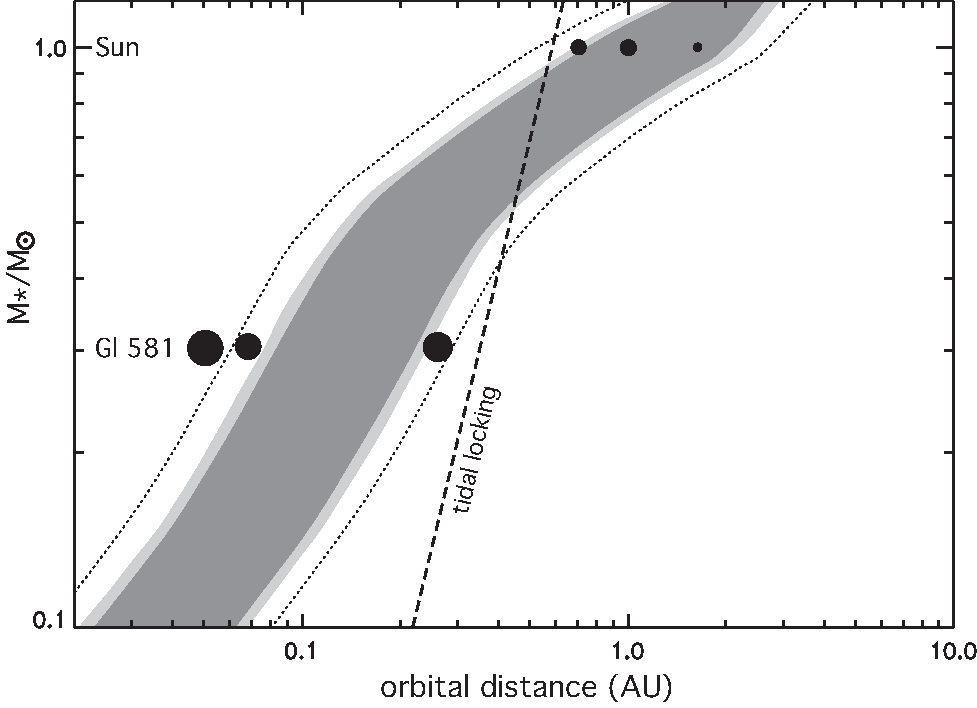
\includegraphics[width=\textwidth]{8091fig3.pdf}
\caption{A plot showing the habitable zone that would remain continuously habitable for at least 5 Gyr (shaded area). The dashed line represents the distance a 1 $M_{\oplus}$ exoplanet would become tidally locked in less than 1 Gyr. Taken from \citet{2007Selsis}.}
\label{FigTidalHZ}
\end{figure}
Tidal forces also apply to the star from the exoplanets gravity, albeit at much smaller magnitudes. These tidal forces can effect the exoplanets orbit, reducing the eccentricity until it is in a circular orbit. As the orbit changes, orbital energy is converted into tidal energy and this causes significant internal heating to occur. The tidal heating rate, taken from \citep{2008Jackson}, is shown in Equation \ref{EqHeat}, where $M_\star$ is the mass of the star, $R_p$ is the radius of the exoplanet, $a$ is the semi-major axis, $e$ is the orbital eccentricity and $Q_p^\prime$ is the corrected tidal dissipation factor. $Q_p^\prime$ is related to $Q$ from Equation \ref{EqTidal} via a correction factor to compensate for the uncertainty in $k$ which leads to an uncertainty in $Q$ \citep{2008Jackson2,1966Goldreich}.\\
\begin{equation}
h = \left(\frac{63}{16\pi}\right) \frac{(GM_\star)^{3/2} M_\star R_p^3}{Q_p^\prime} a^{-15/2} e^2 
\label{EqHeat}
\end{equation}
This heating is strongly dependent on the semi-major axis and to a lesser extent, the eccentricity of the exoplanets orbit. This means that the heating is more significant in a more eccentric orbit but reduces as the orbit becomes more circular. Tidal heating is thought to not only contribute to the overall temperature of the exoplanet, via a transfer of heat through the crust, but also to the formation of planetary atmospheres. During the formation of an exoplanet, particles that are sufficiently close to the protoplanet will become gravitationally bound and will be the precursor to the exoplanets atmosphere. Erosion of these atmospheric gases, through thermal escape and solar winds, can occur at a significant rate. For M-dwarfs, the erosion can be substantial due to habitable zone exoplanets orbiting close to the star. This close proximity will provide the atmospheric gases with additional energy to escape the gravitational pull of the exoplanet and the intensity of the solar wind will be stronger (see Section \ref{SecVar} for more details). By increasing internal convection, tidal heating can increase the rate at which gases, that were trapped in the mantle of an exoplanet, can escape and replenish the atmosphere \citep{2011Perryman}. At high levels ($h\sim0.04$; \citealt{2008Jackson}), tidal heating is predicted to drive plate tectonics, even to the point of possibly making the surface of the planet uninhabitable due to volcanic activity (h\,$>$\,2; \citealt{2008Jackson}).\\

While there are forms of life that can survive in the extreme conditions of gas giants (extremeophiles), when we consider habitability, we are most interested in rocky exoplanets like Earth that can support human life. The mass limit that separates rocky exoplanets from gas giants was initially expected to be around 10 - 15 M$_{\oplus}$ \citep{2006Basri}, from observation of planets in our own solar system. However, due to the discovery of an exoplanet with a mass similar to Saturn but at two thirds the radius \citep{2005Sato}, this limit is in doubt. Methods to obtain a more conclusive limit are being investigated, including using transits \citep{2015Barnes}. Also, there is evidence to suggest there is a third form of exoplanet, with a lower density and gas envelopes of hydrogen and helium. \citet{2014Buchhave} designated high-density rocky planets to have a radius of less than 1.7 R$_{\oplus}$, gas dwarf planets between 1.7 and 3.9 R$_{\oplus}$, and greater than 3.9 R$_{\oplus}$ would be ice/gas giants. 
\section{Variability}
When we look for exoplanets that have the potential to support life, variability of the host star can be an important aspect of a habitability study of any given exoplanet. Not only can stellar activity effect habitability, but it can also hamper exoplanet detection methods. Around 60\% of dwarfs of spectral types $>$ M5 show significant chromospheric activity \citep{1996Hawley}, even during their main sequence lifetimes \citep{2009Kowalski}.\\

The movement of plasma through photospheric convection will induce a magnetic field that can produce localised changes in the star's magnetic field. This plus differential rotation (different parts of the star rotate at different velocities, depending on latitude) can produce magnetic activity such as starspots and flares. This activity has been observed in the Sun and found to be periodic. A study of 99 stars over an 11 year observing campaign starting in 1966 \citep{1968Wilson,1978Wilson}, looked at variations in Ca\,\textsc{ii} H \& K lines and concluded that similar activity cycles were also present in the majority of main sequence dwarfs. 
\subsection{Variability and habitability}
\label{SecVar}
Chromospheric activity can be hazardous to the habitability of exoplanets nearby the star. Convective regions dominate stellar interiors, with stars later than M4 being fully convective. This convection can induce a stellar magnetic field which can cause the star to develop starspots, flares and coronal mass ejections. The intensity of the activity an exoplanet will experience is proportional to its distance from the chromosphere. Therefore, if the habitable zone is sufficiently close to the star, exoplanets within that habitable zone may encounter high levels of activity and be uninhabitable.\\

M-dwarfs are found to be less magnetically active with age \citep{2008West} suggesting that suitability for life might be possible later in the stars lifecycle.\\

\begin{figure}
    \centering
    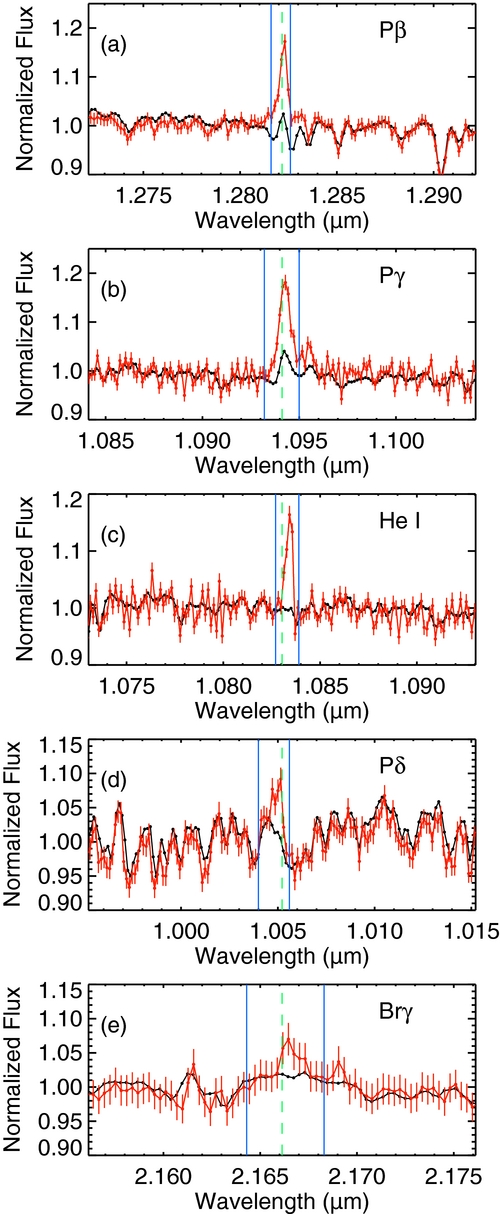
\includegraphics[width=\textwidth,height=0.95\textheight,keepaspectratio]{Flare.jpg}
    \caption{Spectra of EV Lac, taken from \citet{2012Schmidt}. Quiescent (non flaring) spectra is in black while exposures taken while the star was flaring are in red.}
    \label{figFlare}
\end{figure}
Starspots are regions of the photosphere of a star in which the magnetic field is strongly concentrated. This can suppress convection in the area and reduce the surface temperature. The change in temperature can be up to 2000 K in late F and early G stars and 200 K for M stars \citep{2009Strassmeier}. They can be observed as dark regions on the surface of the star that can move position over time. Starspot coverage in M-dwarfs can be as high as 40\% \citep{2004AONeal}. As temperature has a strong influence on habitability, these temperature changes could have a significant impact on the habitability of any exoplanets orbiting a star experiencing starspots.\\

Flares occur when charged particles interact with stellar plasma. They can be observed as a flux increase of several magnitudes across a wide range of wavelengths \citep{2012Schmidt} and a significant increase in emission line strength. For example, the highlighted line in Figure \ref{figFlare} is up to 20\% stronger while the star is flaring. In M-dwarfs the emissions can last for a few minutes to hours \citep{2011Hilton}. Afterwards, the flux returns to normal. While the duration of a flare is relatively short, they have been shown to be quite frequent in some active stars. \citet{2014Hawley} analysed M-dwarf Kepler data and found that the number of flares per day was inversely proportional to the strength of the flares. Emission lines from hydrogen, helium, calcium and iron are commonly used to measure flares \citep{2005Reid}.\\

Often flares will cause the corona to expel radiation and highly energetic particles into space, known as a coronal mass ejection. The high density plasma coming from a coronal mass ejection, at the close distances expected from habitable zone M-dwarf exoplanets can have a strong influence on the exoplanets atmosphere, especially if they are tidally locked and have little or no magnetic moment. The magnetosphere can be compressed, allowing the atmosphere to expand to the point that a substantial fraction can be stripped away \citep{2007Lammer}.
\subsection{Variability and planet detection}
\label{SecActivity}
In addition to disrupting conditions suitable for life on an exoplanet, variability can also interfere with our ability to detect the presence of an exoplanet.\\

Doppler noise, commonly called ``jitter'', is the combination of a number of physical mechanisms that contribute to the intrinsic variability of a host star. It can vary from timescales of 1\,-\,4 days (stellar oscillations) to weeks (granulation and super granulation) to months (star spots) and can cause fluctuations in Doppler velocity measurements of 3.5\,-\,5 ms$^{-1}$ for cool stars like M-dwarfs \citep{2005Wright}.\\

During the mid 1990's, the ELODIE spectrograph \citep{1996Baranne} was designed to be as stable as possible using the technology of the time. ELODIE initially achieved a precision of $\sim$13 ms$^{-1}$. At this level, only objects with large Doppler velocity amplitudes (e.g. Jupiter-sized exoplanets) were detectable and stellar activity was not as significant a source of noise at these amplitudes. Modern technology has delivered better stability and better velocity precision - the HARPS spectrograph \citep{2010Wright} has been able to detect Doppler velocities with a precision of 1 ms$^{-1}$ \citep{2011Dumusque}. Unfortunately, since variations due to activity from an active star can have similar amplitudes, activity can produce false detections for exoplanets.\\

Periodic variability, such as starspots, can be mistaken for orbiting exoplanets that have orbital periods up to hundreds of days. \citet{1997Saar} modelled starspots on G type stars and found that the amplitude of the Doppler velocity variations due to starspots was proportional to the fraction of the surface area of the star that the starspots inhabit, $f_s$, and the rotational velocity of the star, $v sin(i)$. Thus, fast rotating stars will have their Doppler velocities affected by starspots more than slower rotating stars.\\

\subsubsection{Quantifying variability}
\label{SecVarMeth}
The standard practice for measuring the variability of a star is through Line Profile Variations (LPV). Several absorption lines have been identified that are known to contain emission features at their cores. These emission features vary over time, in proportion to the level of variability in the star. An example of this is Figure\,\ref{figNaD_line} in which an emission feature can be clearly seen to vary over a number of observations. \citealt{1978Wilson} first correlated flux across the Ca\,\textsc{ii} H (3968.47\,\AA) \& K (3933.66\,\AA) lines to chromospheric activity by looking at the spectra of 91 main sequence stars over a roughly 10 year period. For most stars, these lines are used to measure variability. However as the wavelength distribution of a star's flux varies with its temperature, the amount of flux across the Ca\,\textsc{ii} H\,\&\,K lines will also vary. As M-dwarfs have the majority of their flux in the near-IR, the Ca\,\textsc{ii} H \& K lines are weaker than in hotter stars and, while still useful, are not as useful as other lines as suitable proxies for variability. Specifically, the H\,\textsc{$\alpha$} (6562.808\,\AA) and Na\,\textsc{i} D lines (5895.92\,\AA\,\& 5889.95\,\AA).\\

\begin{figure}
    \centering
    \includegraphics[width=0.8\textwidth]{NaD_example.png}
    \caption{Spectra of GL803, focusing on one of the Na\,\textsc{i} D lines. An emission feature can be seen in the centre of the absorption feature, which varies from observation to observation.}
    \label{figNaD_line}
\end{figure}

Additionally, each of these lines has been found to measure chromospheric activity at different altitudes. Ca\,\textsc{ii} H \& K measures activity in the lower levels, Na\,\textsc{i} D for the middle-to-lower levels, and for the upper levels, H\,\textsc{$\alpha$}.\\

A stellar activity index is measured as the sum of the flux across a ``window'' of wavelengths, centred on the line of interest, divided by the flux in the continuum around the line. For example, the Mount Wilson S-index \citep{1978Vaughan} uses the flux in the Ca\,\textsc{ii} H line, $N_H$, and K line, $N_K$, divided by the flux on the violet, $N_V$, and red, $N_R$, sides of the two lines in Equation \ref{eqSind}.
\begin{equation}
	S = \frac{N_H + N_K}{N_V + N_R}
	\label{eqSind}
\end{equation}


A stellar activity index can be measured for multiple observations and any periodic variability in the stellar activity index can be identified and compared with periodic variations found in the Doppler velocity of the star. Doppler velocities that vary with a similar velocity to the stellar activity index variations are most likely to be due to stellar activity, rather than an exoplanet.
\begin{figure}
    \hspace{-1cm}
    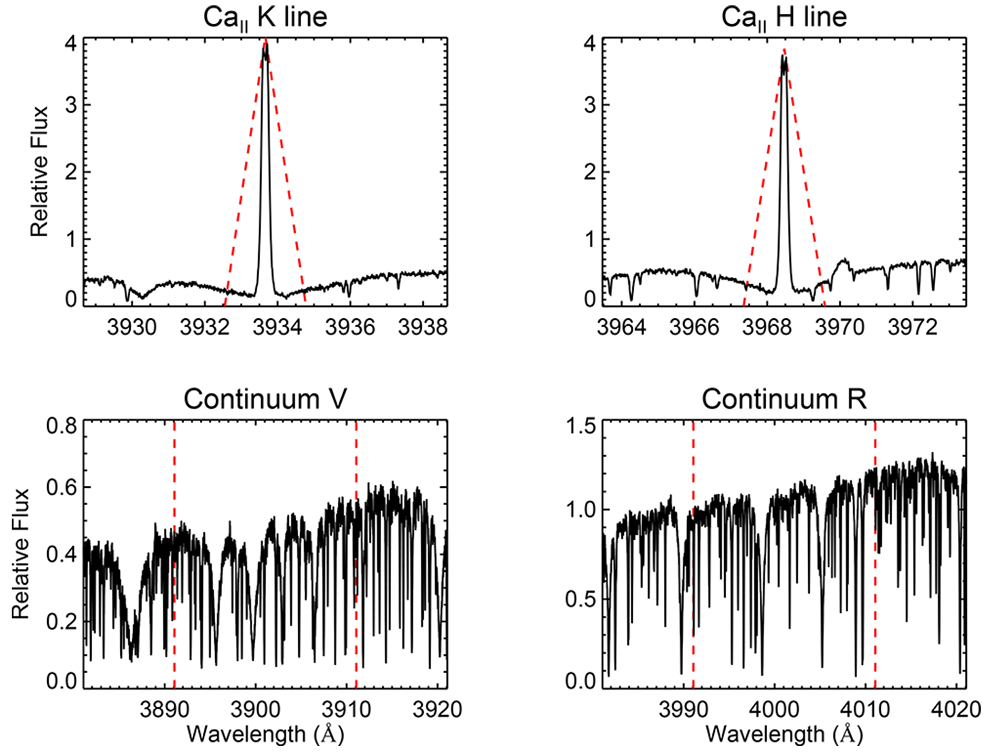
\includegraphics[scale=0.5]{MtWilson.png}
    \caption{Total flux within the red dashed lines are used to determine the Mount Wilson S-index (Equation\,\ref{eqSind}). The upper left and right regions indicate $N_K$ and $N_H$ respectively, and the lower left and right regions determine $N_V$ and $N_R$. Figure taken from \citet{2015Suarez}.}
    \label{figLPVexample}
\end{figure}
